\pagebreak
\subsubsection{Hierarchical Cluster}

En la figura \ref{fig:cluster} se muestran las tablas de confusión obtenidas con el algoritmo de Hierarchical cluster usando un linkage de tipo complete con una distancia coseno para los años 2015 y 2020.

\begin{figure}[H]
    \centering
    \begin{subfigure}{8.4cm}
        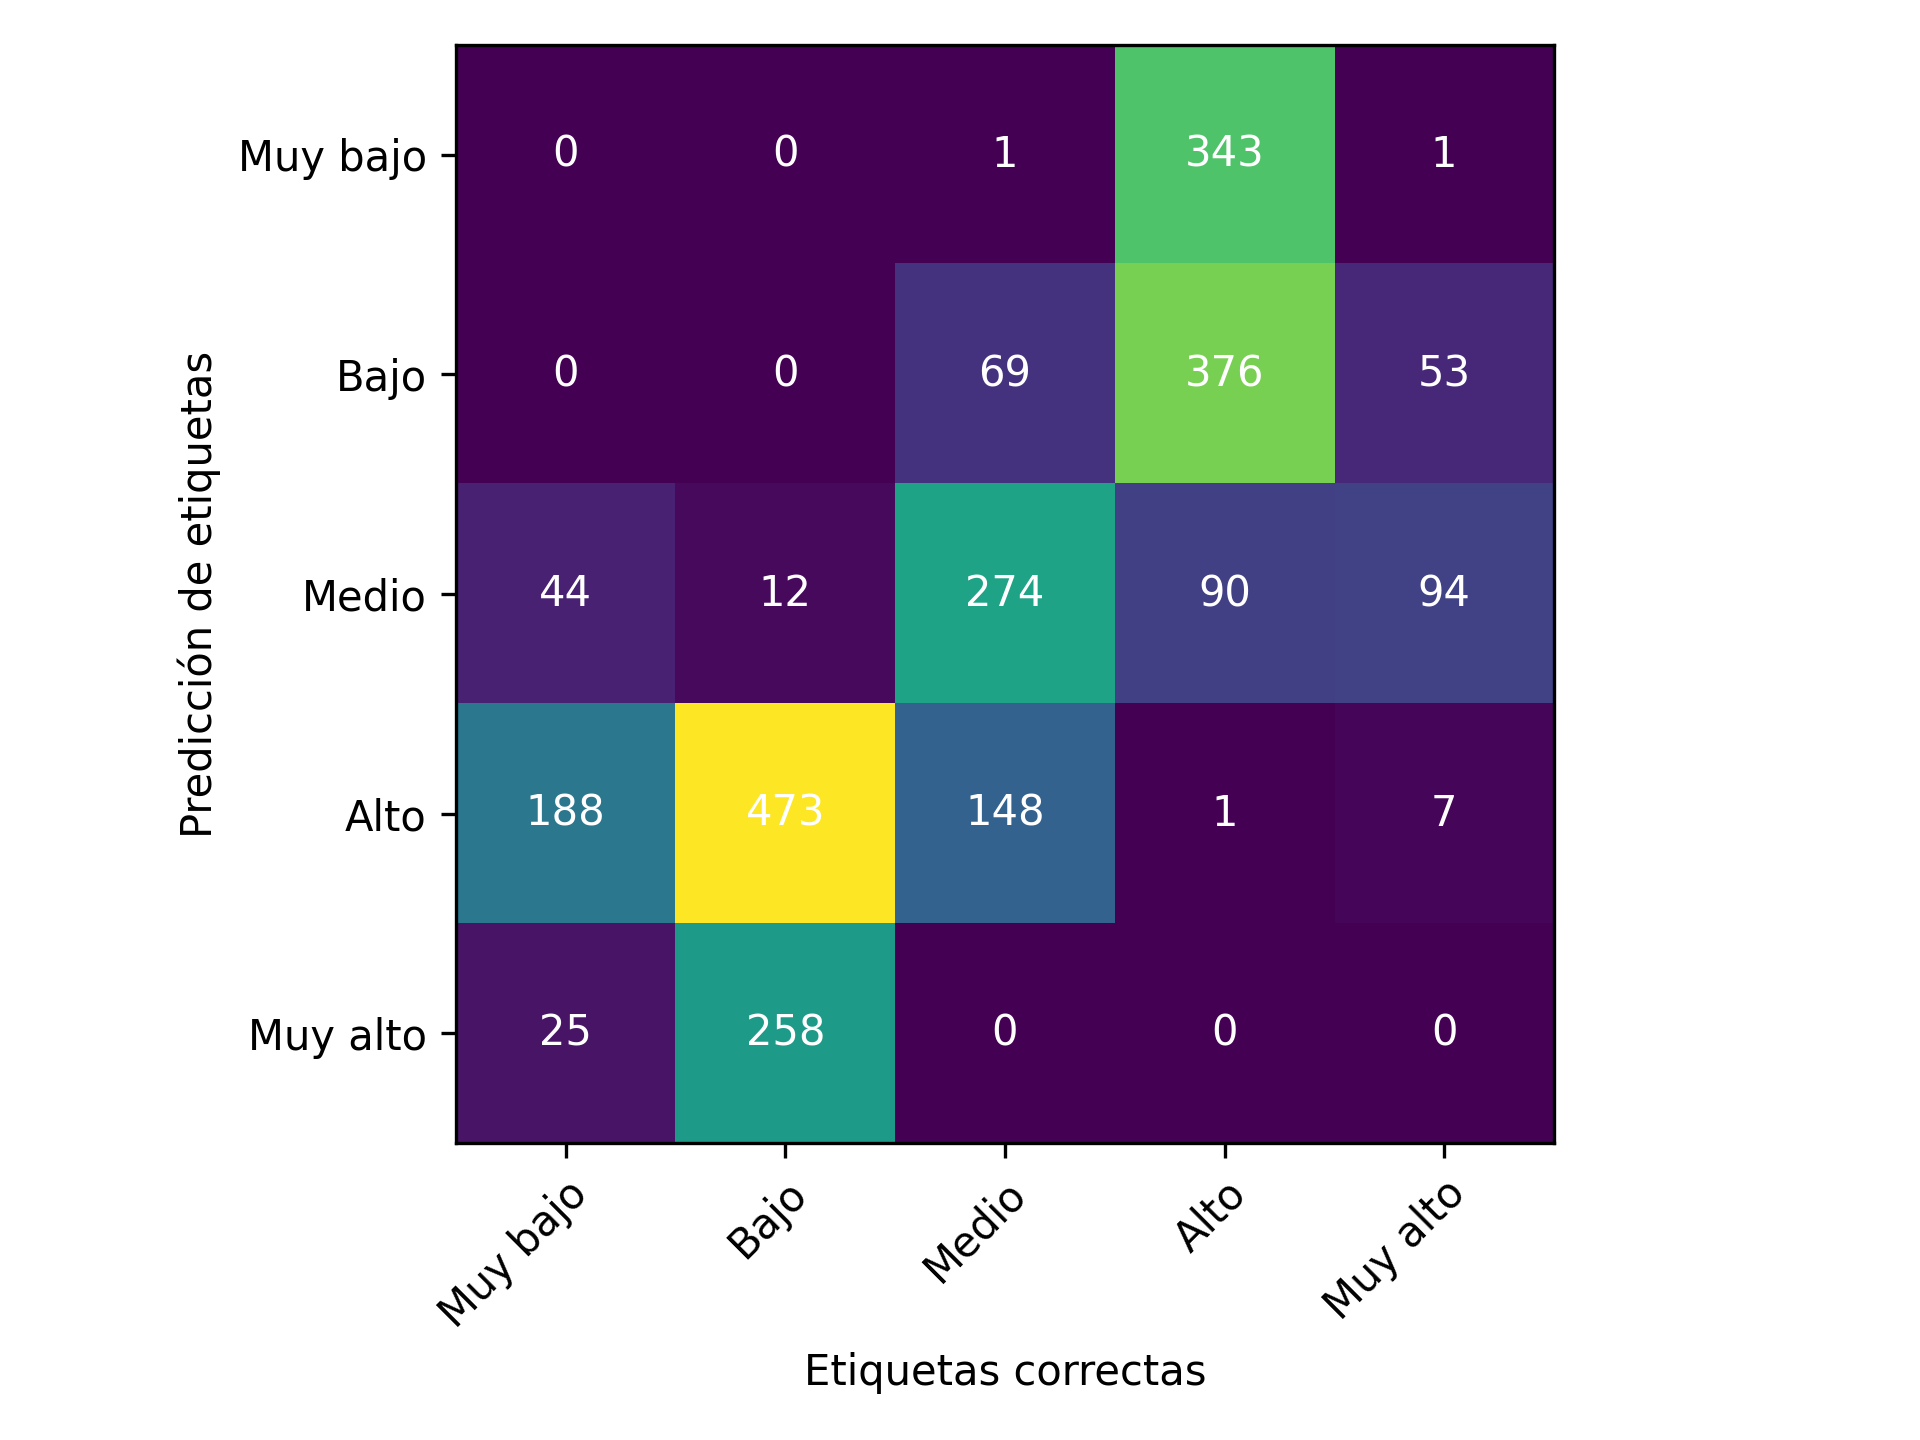
\includegraphics[width=1\linewidth]{Graphics/Data_2015/Cluster_confusion_matrix.png}
        \caption{Año 2015}
    \end{subfigure}
    \begin{subfigure}{8.4cm}
        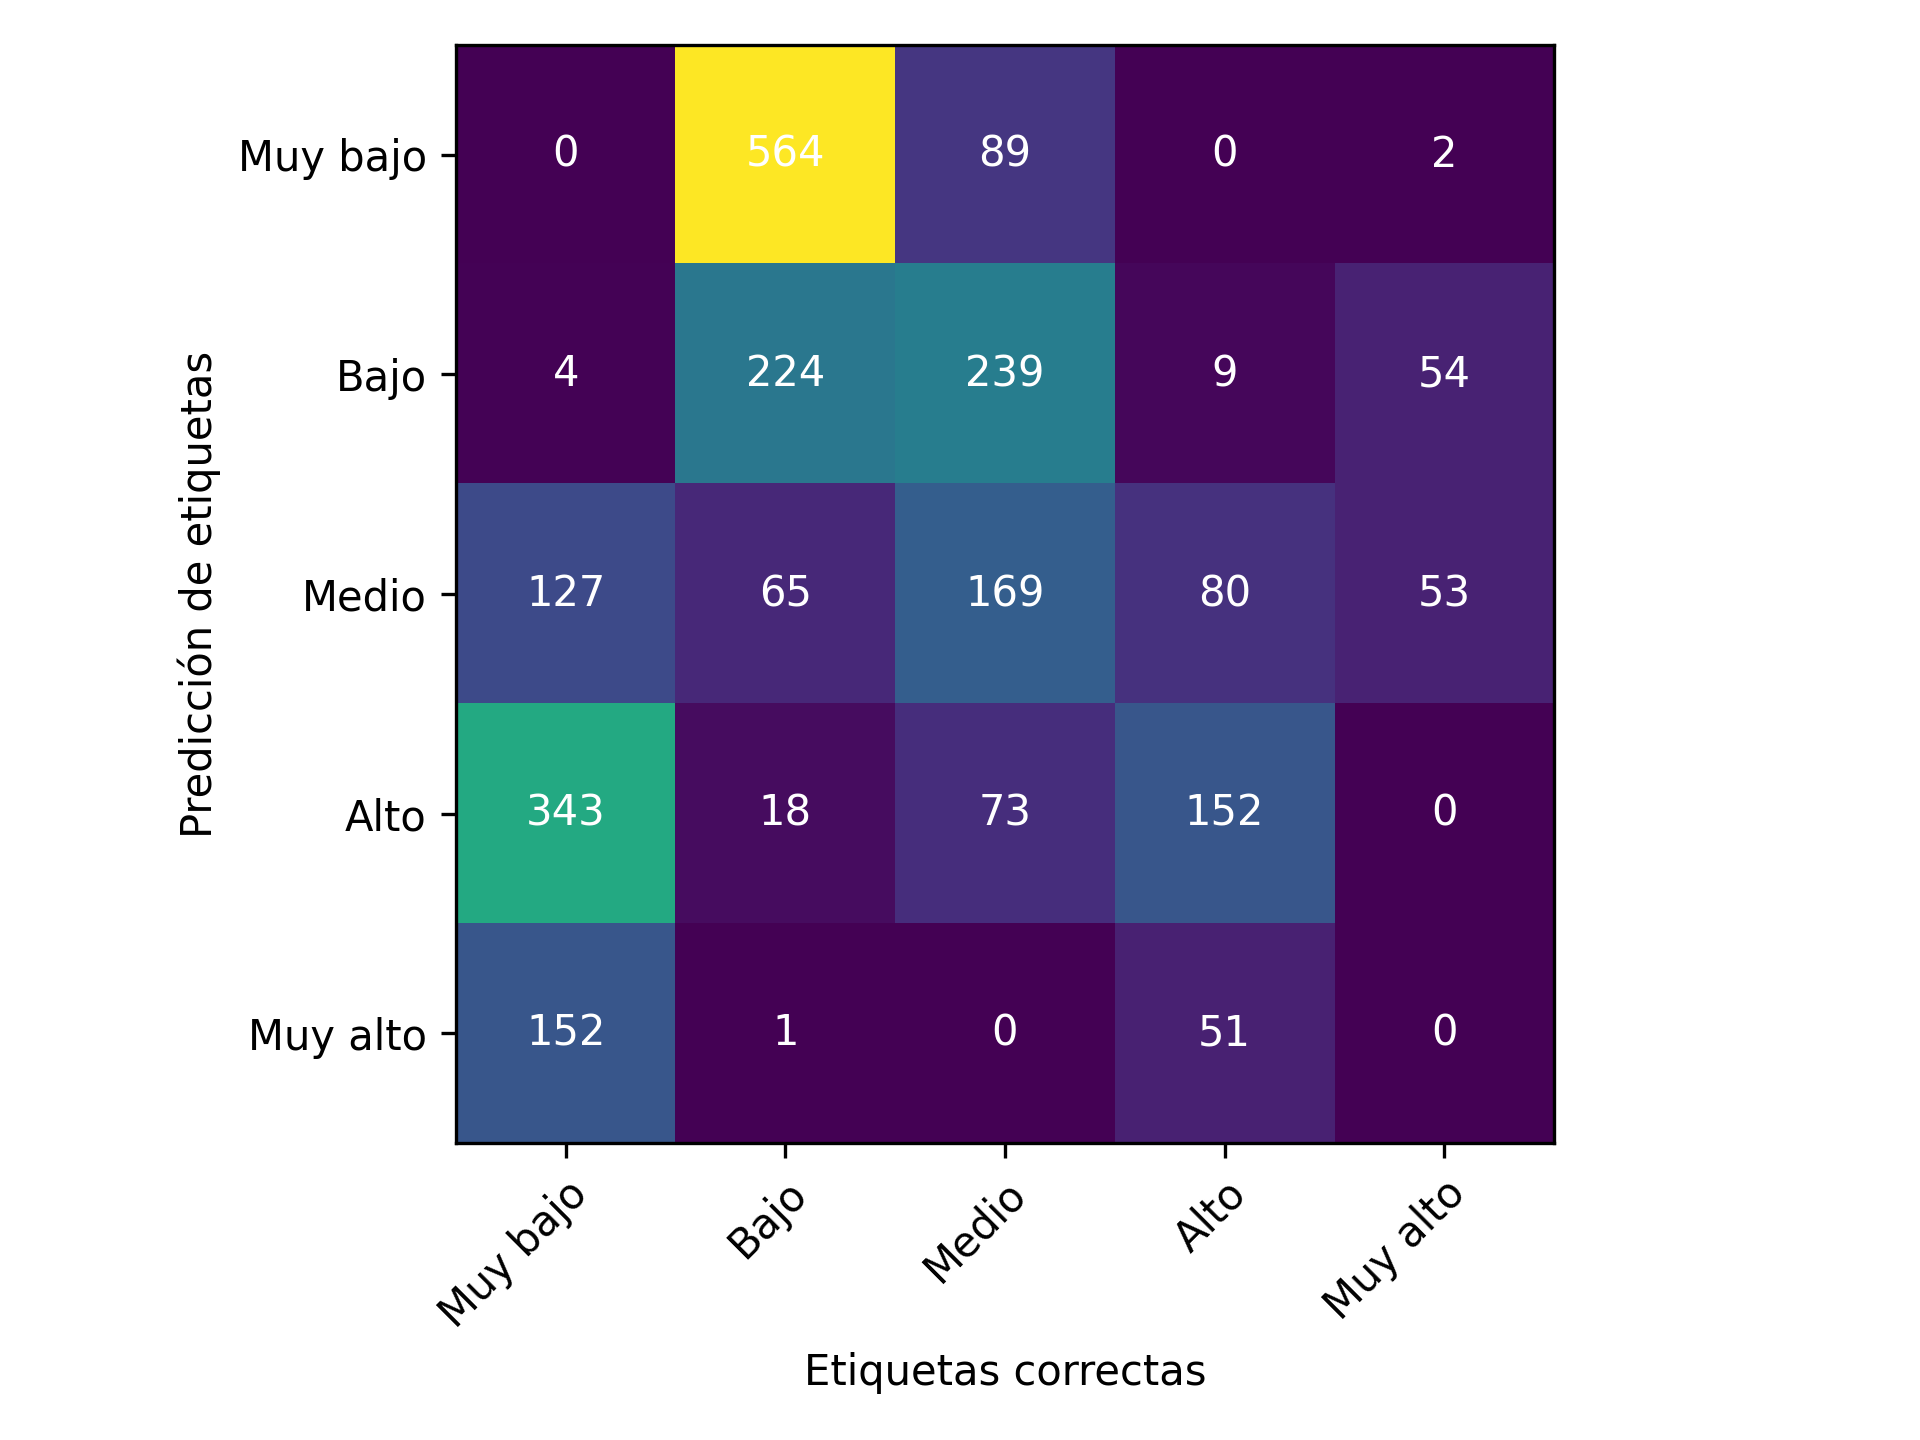
\includegraphics[width=1\linewidth]{Graphics/Data_2020/Cluster_confusion_matrix.png}
        \caption{Año 2020}
    \end{subfigure}
    \caption{Matrices de confusión resultantes del algoritmo Hierarchical cluster para los años 2015 y 2020.}
    \label{fig:cluster}
\end{figure}